\documentclass[12pt,polish,a4paper, left=254mm, right=254mm, top=150mm, bottom=150mm]{report}
% Importy paczek
\usepackage{amsmath, amssymb, amsthm}
\usepackage{pgfplots}
\usepackage{polski}
\usepackage[polish]{babel}
\usepackage[T1]{fontenc}
\usepackage[utf8]{inputenc}
\usepackage{graphicx}
\usepackage{array}
\usepackage{pgfplots}
\usepackage{pdfpages}
\usepackage{fancyvrb}
\usepackage{mathptmx}

% Makro do rozmiaru customowego czcionki
\newenvironment{localsize}[1]
{%
  \clearpage
  \let\orignewcommand\newcommand
  \let\newcommand\renewcommand
  \makeatletter
  \input{bk#1.clo}%
  \makeatother
  \let\newcommand\orignewcommand
}
{%
  \clearpage
}

% Import bitex i dodanie źródła z bibliografią
\usepackage[backend=bibtex,style=numeric,sorting=none]{biblatex}
\addbibresource{References.bib}

% Ścieżka do grafiki
\graphicspath{{images/}}

% Importy paczek upiększających
\usepackage{float}

% Makro dla opis+źródło
\begin{document}
\newcommand*{\captionsource}[2]{%
  \caption[{#1}]{%
    #1 %
    % \hspace{\linewidth}%
    (Źródło: #2)%
  }%
}

% Strona tytułowa
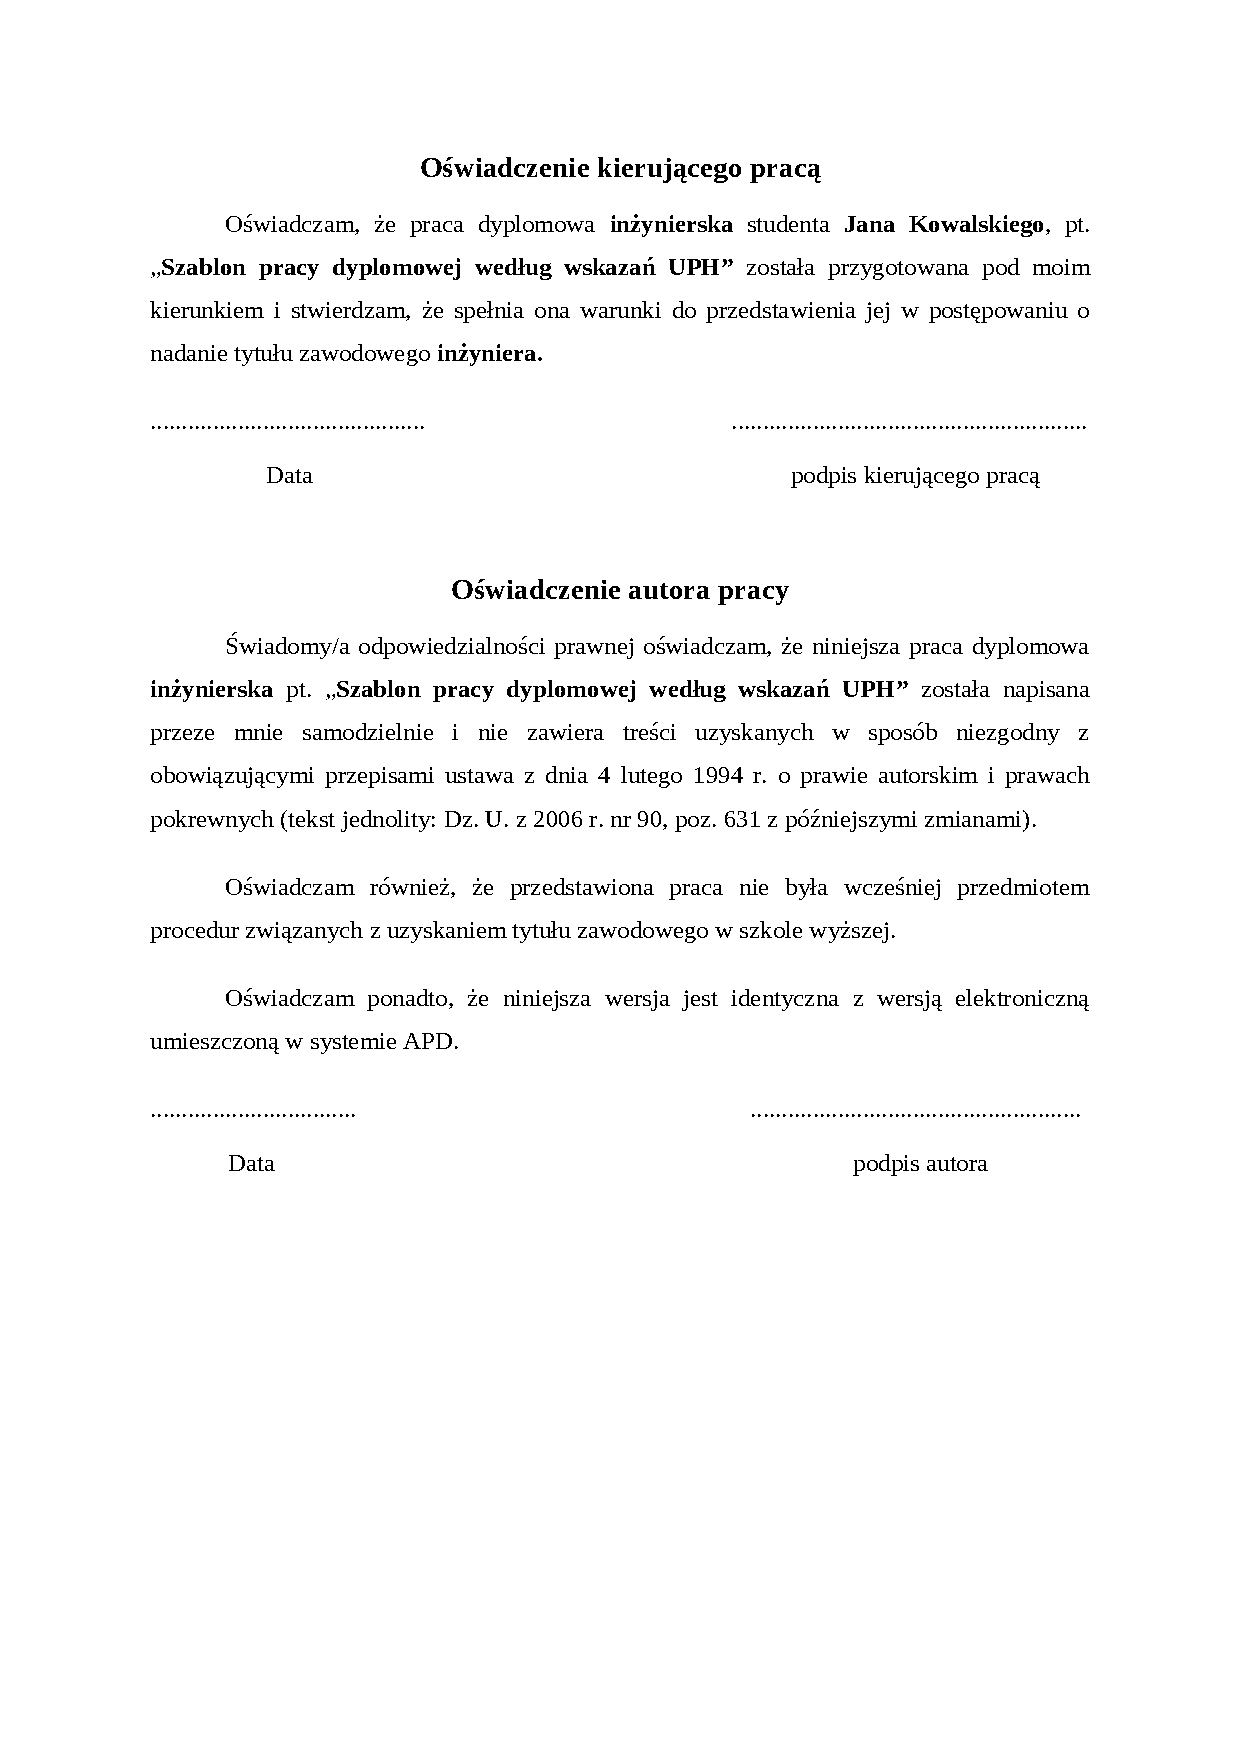
\includepdf[pages=-]{oswiadczenie_i_tytulowa.pdf}

% Tytuł pracy i słowa kluczowe PL/EN
\subsection*{Tytuł pracy inżynierskiej w języku polskim:}


\textit{``Szablon pracy dyplomowej według wskazań UPH''}

\subsection*{Wykaz słów kluczowych w języku polskim:}

\begin{enumerate}
  \item Słowo 1
  \item Słowo 2
  \item Słowo 3
\end{enumerate}

\subsection*{Tytuł pracy inżynierskiej w języku angielskim:}

\textit{``Szablon pracy dyplomowej według wskazań UPH''}

\subsection*{Wykaz słów kluczowych w języku angielskim:}

\begin{enumerate}
  \item Słowo 1
  \item Słowo 2
  \item Słowo 3
\end{enumerate}



\setcounter{tocdepth}{1}
\tableofcontents

\chapter*{Wstęp}
\addcontentsline{toc}{chapter}{Wstęp}
Tutaj napisz swój wstęp.


% <<< ======================================================================================== <<<
% Tutaj wklejaj swoje rozdziały

\chapter{Rozdział pomocniczy do utworzenia pracy dyplomowej}
Ala ma kota a kot ma alę.

\section{Referencje, Obrazki, wzory i wykresy}

\subsection{Referencje}

``Super referencja wow ale super!''\cite{rosenblatt1962principles}.

\subsection{obrazek}
Przykład obrazka:

\begin{figure}[H]
	\centering
	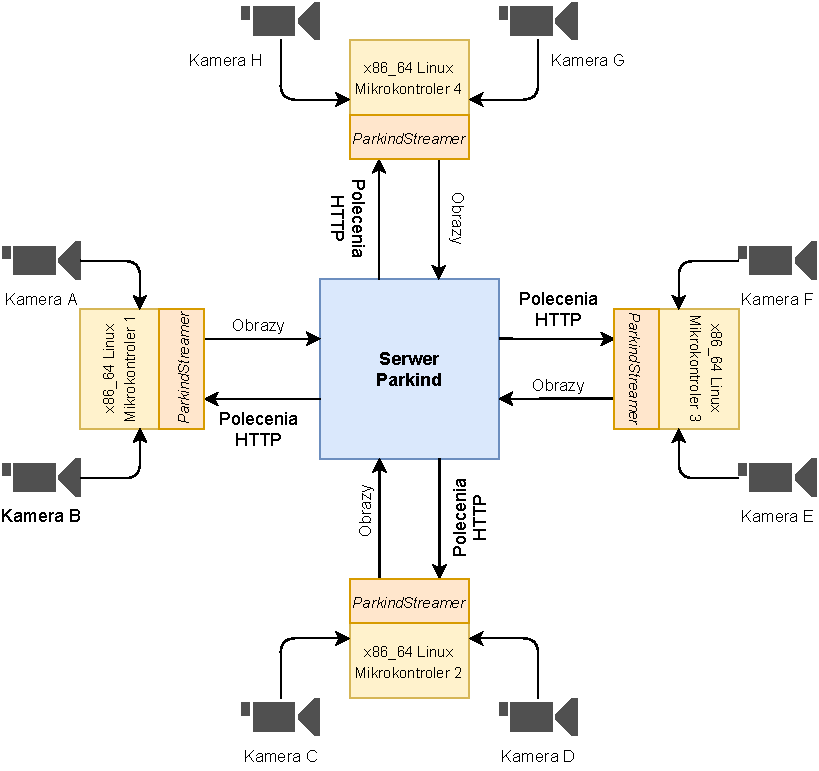
\includegraphics[width=0.5\columnwidth]{Graphics/Chapter 2/Parkind Network Topography.pdf}
	\captionsource{Topografia sieci Parkind}{Opracowanie własne}
	\label{fig:2ch1}
\end{figure}

\subsection{wzór}

Przykład wzoru:

\begin{equation}
	y = f(g(x)) =
		\begin{cases}
			1	&\textit{jeśli g(x)}\geq\theta \\ % 
			0	&\textit{jeśli g(x)}<\theta % 
		\end{cases}
\end{equation}

\subsection{wykres}

Przykład wykresu:

\begin{figure}[H]
   	\centering
	\begin{tikzpicture}
		\begin{axis}[x=1cm, y=1cm,
			axis lines=middle,
			xlabel=$\sum_{i=1}^nw_{i}x_i$, % =\sum_{i=1}^nw_{i}x_i
			ylabel=\(y\), 
			x label style={anchor=north}, % kierunek osi X
			y label style={anchor=east}, % kierunek osi 
			xmin=0, xmax=9, ymin=0, ymax=6, % do którego momentu i od którego momentu ma być pokazywana funkcja
			xtick={0,...,8},
			xticklabel=\empty, % bez liczb
			yticklabel=\empty,
			ytick={0,...,5},
			clip=false, % nwm co to
			domain=0:3]

			% \addplot[red] {ifthenelse(x<4, 0, 1)}; % node[right]{$\tanh x$};
			\addplot[blue, thick] coordinates {(0,0) (1,0) (2,0) (3,0) (3.999999, 0) (4, 5) (5, 5) (6, 5) (7, 5) (8, 5)};
		\end{axis}
		% \node[font=\color{black}] at (4,-0.25) {$-w_0$};
		\node[font=\color{black}] at (4,-0.3) {$\theta$};
		\node[font=\color{black}] at (-0.25, 0) {$0$};
		\node[font=\color{black}] at (-0.25, 5) {$1$};
	\end{tikzpicture}
	\captionsource{Wykres funkcji progowej}{Opracowanie własne}
    \label{fig:2ch2}
\end{figure}

\section{Tablice i skrawki kodu źródłowego}

Przykład tablicy:

\begin{table}[H]
	\centering

    \begin{center}
        \begin{tabular}{ | m{3.2cm} | m{1.75cm} | m{2cm} | m{5cm} | } \hline
            \textbf{URL} & \textbf{Metoda} & \textbf{Ciało} & \textbf{Cel Użycia} \\
            \hline
            \hline
            /\textit{entity}/list & GET & (Puste) & Pobranie listy obiektów \textit{entity} w bazie danych parkind \\
            \hline
            /\textit{entity}/detail/\textit{id} & GET & (Puste) & Pobranie szczegółowych informacji nt. danego obiektu \textit{entity} \\
            \hline
            /\textit{entity}/create/ & POST & entity w formie JSON & Utworzenie obiektu \textit{entity} przy użyciu podanych danych \\
            \hline
		/\textit{entity}/update/\textit{id} & PUT & entity w formie JSON & Zaktualizowanie istniejącego obiektu \textit{entity} przy użyciu podanych danych \\
            \hline
            /\textit{entity}/delete/\textit{id} & DELETE & (Puste) & Usunięcie istniejącego obiektu \textit{entity} przy użyciu podanego numeru identyfikacyjnego \\
            \hline
        \end{tabular} \\ 
        % \hfill \\
    \end{center}

	\captionsource{Operacje CRUD w Parkind API gdzie \textit{entity} oraz \textit{id} są zmiennymi przedstawiającymi odpowiednio typ oraz identyfikator obiektu}{Opracowanie własne}
	\label{Tab:2tb1}
\end{table}

Skrawek kodu źródłowego:

\begin{figure}[H]
    \centering
    \begin{Verbatim}[numbers=left,xleftmargin=5mm]
// Utwórz serwer http i połącz z serwerem Parkind pod adresem "addr"
addr := "127.0.0.1"
server, camSession, err := streaming.CreateHTTPServer(true, addr)

// Jeżeli zaszedł błąd przerwij wykonywanie
if err != nil {
	logging.ErrorLog(err.Error())
	os.Exit(1)
}
    
// Pod koniec programu zamknij serwer i sesję odczytu z kamery
defer camSession.Close()
defer server.Close()

// Rozpocznij działanie serwera
err = server.ListenAndServe()
if err != nil {
	logging.ErrorLog(err.Error())
	os.Exit(2)
}
	\end{Verbatim}
    \captionsource{Kod przedstawiający działanie modułu przesyłu}{Opracowanie własne}
    \label{code:2ch1}
\end{figure}






\chapter*{Podsumowanie oraz wnioski}
\addcontentsline{toc}{chapter}{Podsumowanie oraz wnioski}
Mój super system jest najelpsiejszy.



\addcontentsline{toc}{chapter}{Bibliografia}
\printbibliography

\addcontentsline{toc}{chapter}{Spis Rysunków}
\listoffigures

\addcontentsline{toc}{chapter}{Spis tabel}
\listoftables

\end{document}

